\subsection{Technologien und Werkzeuge}

\subsubsection{Android Bildschirmaufzeichnung}
Eine der Neuerungen, welche mit Android 4.4 \enquote{KitKat} eingeführt wurde, ist die Möglichkeit den Bildschirminhalt in Form eines Videos aufzuzeichnen.
Die Aufzeichnung wird über einen PC gestartet, der mit dem Android Gerät über die \ac{ADB} \cite{AndroidDevelopers.2014b} per \ac{USB}-Kabel oder kabellos verbunden ist.
Die Aufzeichnung wird mit dem Befehl \texttt{adb shell screenrecord} gestartet werden.
Soll ein Teil einer Applikation nicht aufgezeichnet werden, so kann der Entwickler die Aufnahme mit \texttt{SurfaceView.setSecure()} verhindern.
Die Aufzeichnung wird im MP4"~Format auf dem Gerät gespeichert und lässt sich von dort abrufen, z.~B. mit der \ac{ADB} oder über eine \ac{USB} \ac{MTP}.
\cite[Vgl.][]{AndroidDevelopers.2014}
\begin{wrapfigure}{l}{.3\textwidth}
	\centering
	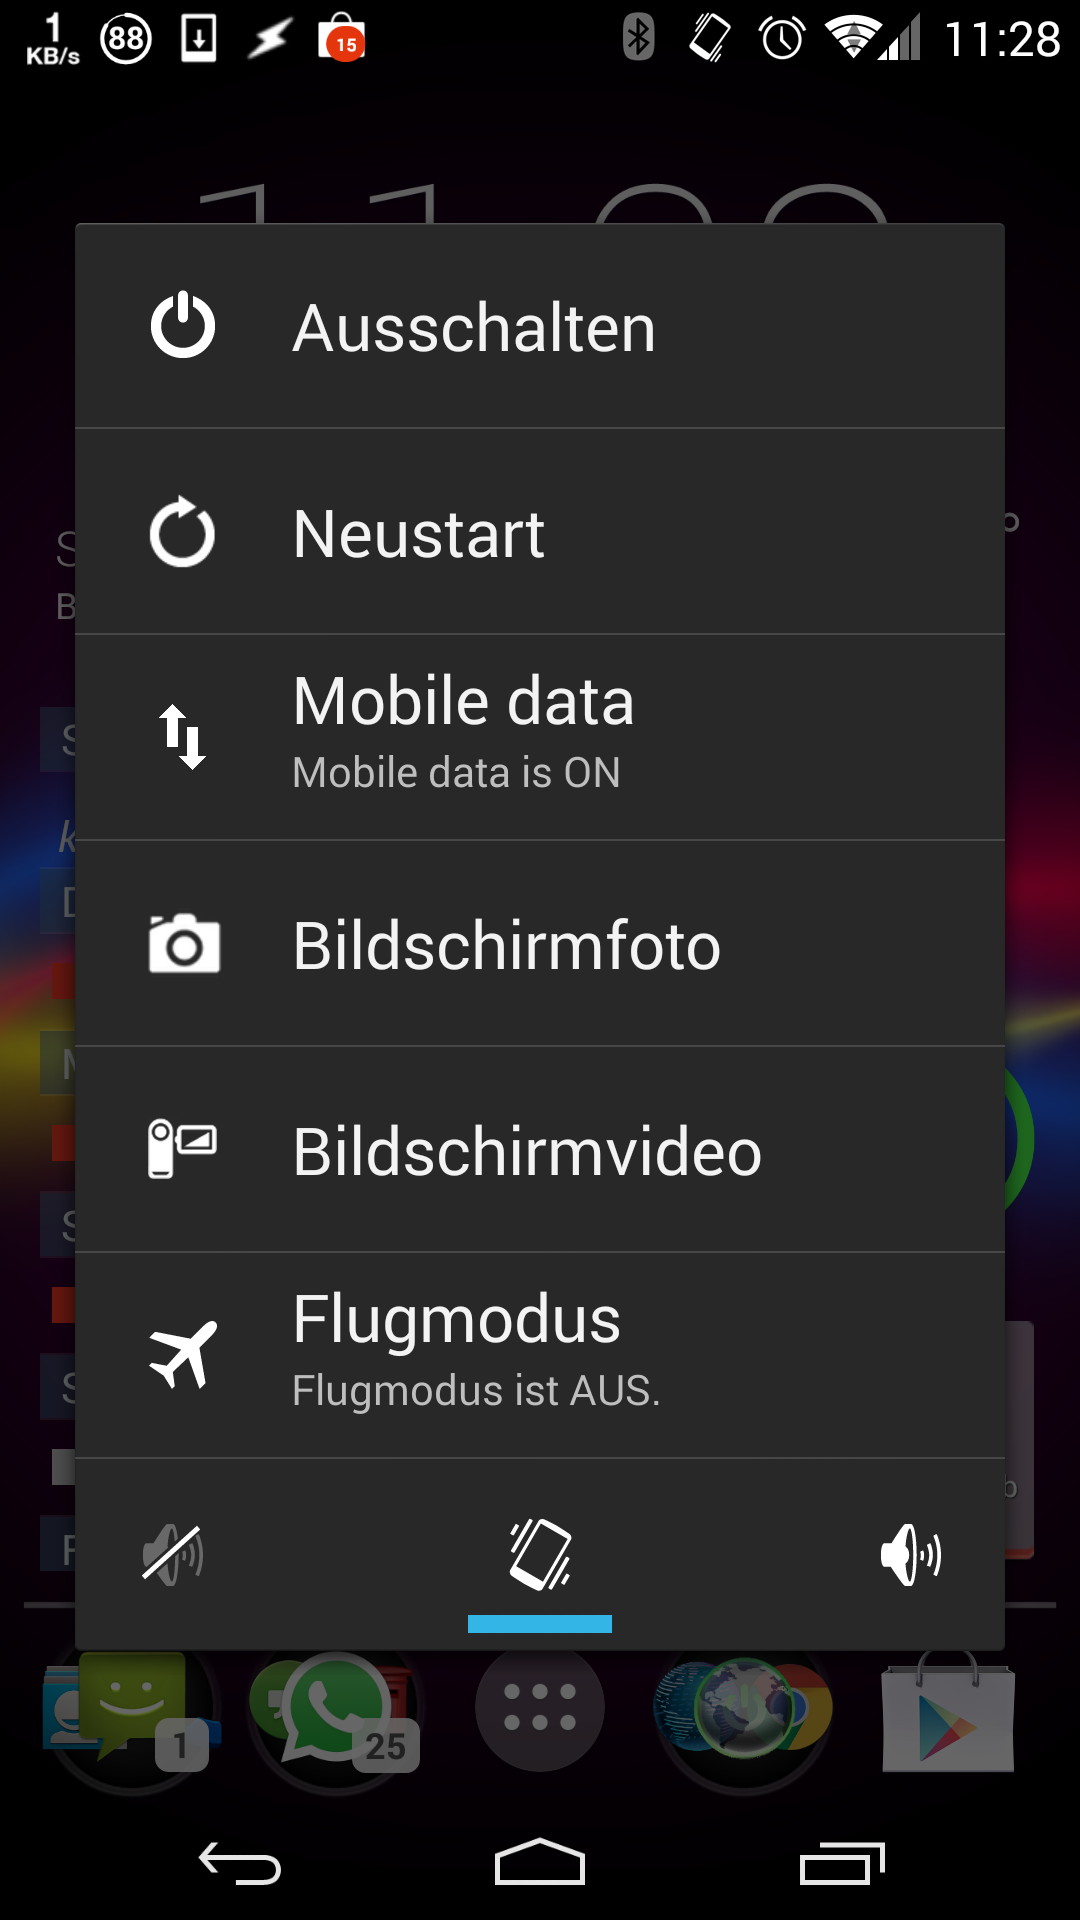
\includegraphics[width=\linewidth]{img/screenshot_omnirom_power_menu}
	\caption{Screenshot des OmniROM Power-Menüs.}
	\label{fig:screenshot_omnirom_power_menu}
\end{wrapfigure}
\ac{ADB} ist ein Debugging-Werkzeug, welches als Bestandteil des Android \ac{SDK} \cite{AndroidOpenSourceProject.2014c} ausgeliefert wird.
Mit ihm lassen sich Befehle direkt auf Shell des Geräts ausführen.
Vor Android 4.4 war es bereits möglich mit dem Befehl \texttt{adb shell screencap -p /sdcard/<name>.png} Bildschirmfotos zu erstellen \cite[vgl.][]{RandomStuff.2013}.
Diese Möglichkeit besteht seit Android 4.0 \enquote{Ice Cream Sandwich} (ICS).

Die beiden genannten Möglichkeiten für Aufzeichnungen des Bildschirminhalts benötigen jedoch einen per \ac{ADB} verbundenen PC.

Um diese Befehle direkt auf dem Gerät aus einer Applikation heraus auszuführen, wird der Root-Zugriff auf dem Gerät benötigt \cite[vgl.][22]{Erxleben.2014}.

Alternativ bieten einige Geräte und sog. \enquote{Custom-ROMs} die Möglichkeit Bildschirmfotos und -videos direkt aus einem Menü heraus oder per Tastenkombination zu erstellen. 
Abbildung \ref{fig:screenshot_omnirom_power_menu} zeigt beispielhaft das Power-Menü von \emph{OmniROM}\footnote{OmniROM Webseite: \url{http://omnirom.org/}}.

Eine Möglichkeit um den Bildschirminhalt auf einem zusätzlichen Display anzuzeigen wird im nächsten Abschnitt kurz erläutert.

\subsubsection{Chromecast Screen Mirroring}
Der Google \emph{Chromecast} ist ein Streaming-Client, welcher z.~B. an Monitoren oder Fernsehern angeschlossen werden kann.
Nach der ersten Einrichtung kann er u.~a. über Android Geräte im selben Netzwerk gesteuert werden.
Applikationen mit \emph{Chromecast} Unterstützung können Medien auf diesem Weg Inhalte direkt auf einem Bildschirm darstellen. \cite[Vgl.][]{Google.2014}
Neben dem Streaming von Medieninhalten aus dem Internet unterstützt die aktuelle \emph{Chromecast} Applikation für Android \cite{GoogleInc..2014} auch das Übertragen des Bildschirminhalts mit sehr geringer Latenz.
Diese Funktion ist allerdings nicht für alle Geräte verfügbar.
Eine Aufzeichnung der Übertragung wird aktuell nicht unterstützt.

Auch wenn es andere Lösungen gibt, um den Bildschirminhalt eines mobilen Geräts zu übertragen, \emph{Chromecast} ist mit 35~\texteuro\xspace \footnote{Preisangabe des Herstellers, Stand: Oktober 2014. Webseite: \url{https://www.google.de/chrome/devices/chromecast/}} einer der preiswertesten Wege, bei dem nur ein Fernseher oder Monitor benötigt wird.
Besonders spannend sind die Möglichkeiten für Labortests, denn die Kamera, welche den Bildschirm abfilmt könnte entfallen und der Testbenutzer kann sich frei im Raum, bzw. in der Reichweite des kabellosen Netzwerks, bewegen.